\chapter{EVALUATION}

The Information Extraction and the Ontology Similarity modules are two important part of the system.  We will evaluate them respectively. 

\section{Experiments of Information Extraction }

To evaluate the performance of information extraction, we get some sentences by the sentence filters, different sentence filter can extract different kinds of sentences. We use degree sentences to explain the process: 
 
In the experiment, we selected 100 sentences from job descriptions that are requirements of candidates degree and major. The value of degree and major are labeled manually. We use patterns to  match and extract the degree information from the sentences. The pattern is gotten from the observation of sentences. As we add more pattern, the accuracy of information increased as well. When we used 6 patterns, the accuracy of degree became 94\%. Figure \ref{fig:degree_accuracy} show the accuracy with number of patterns. 

\begin{figure}[htbp]
  \centering
  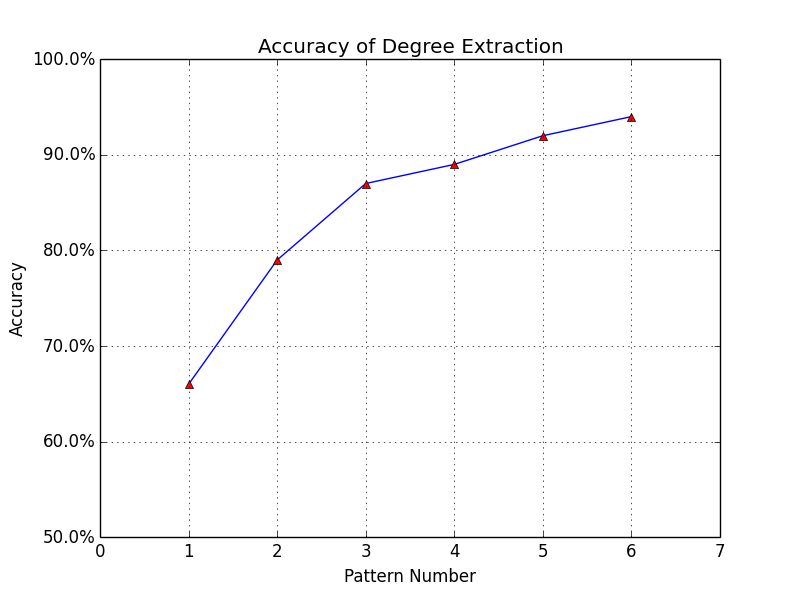
\includegraphics[scale=0.5]{images/degree_accuracy.png}
  \caption{Degree Extraction  Accuracy}
  \label{fig:degree_accuracy}
\end{figure}


\begin{table}[ht]
\caption{Information Extraction} % title of Table
\centering % used for centering table
\begin{tabular}{   | c | c | c | c |   }
 \hline
                     type   & Precision & Recall     \\
 \hline
                     Degree & 0.94      & 0.99         \\
 \hline
                     Degree & 0.94      & 0.99      \\
 \hline
                     Degree & 0.94      & 0.99        \\
 \hline
\end{tabular}
\label{tab:ie} % is used to refer this table in the text
\end{table}


To evaluate the system, some measures will be used. We also proposed two evaluation method: Pre-collected Data and User's direct experience.

\section{Basic measures of the system}

In traditional information retrieval system, some measures are widely used~\cite{manning2008introduction}. These measures include:

\begin{enumerate}
    \item Precision ($P$) is the fraction of retrieved documents that are relevant .
       $$  Precision =  \frac{ \#(releveant~items~ retrieved)}{ \#(retrieved~items)}$$
    \item Recall ($R$) is the fraction of relevant documents that are retrieved.
       $$  Recall =  \frac{ \#(releveant~items~ retrieved)}{ \#(releveant~items)}$$
    \item $F measure$ ($F_1 score$) trades off precision versus recall.
       $$ F_1 = 2 \cdot \frac{ Precision \cdot Recall}{ Precision + Recall } $$
    \item Since the results are ranked, $ Normalized~Discounted~Cumulative~Gain ( NDCG )$ will be an important measure to evaluate the ranked retrieval results. For a set of queries $Q$, let $R(j,d)$ be the relevance score assessors gave to document $d$ for query $j$.
       $$ NDCG(Q,k) = \frac {1}{|Q|} \sum_{j=1}^{|Q|}{Z_{kj}} \sum_{m=1}^{k} \frac{2^{R(j,m)} - 1}{ \log_2(1+m)} $$
where $Z_{kj}$ is a normalization factor calculated to make it so that a perfect ranking's NDCG at $k$ for query $j$ is 1. For queries for which $k' < k$ documents are retrieved, the last summation is done up to $k'$.

\end{enumerate}

\section{Pre-collected Data}

Some resumes will be pre-collected, and some their matched jobs will be found manually. These jobs will be put into the job database with some other unrelated jobs.  When searching the jobs with the resume, we can get precision, recall and F measure of the system. With ranking positions of the searching results we could calculate the NDCG measure.

\section{Experimental Setup}



\section{Experimental Results}

Given a set of candidates that satisfy the filtering conditions, we would like to display candidates that better match
the job requirements at the top. We create a query q from the job requirements and treat the text of the candidate resumes as documents d and apply standard ad-hoc retrieval techniques to rank the candidates. The different retrieval algorithms we use are Okapi BM25 (from the Lemur toolkit), Kullback{Leibler divergence of language models with Dirichlet smoothing (also from the Lemur toolkit) and the TF-IDF scoring model in Lucene. Since the job descriptions are fairly verbose we also experiment with a retrieval model where certain terms that are important to the quality of the match are weighted up in the TF-IDF scoring model. In our experiments we extracted the skills from the job description using a simple dictionary based extraction method where the dictionary consisted of a set of skills that we extracted using the system described in Section 4 from all the resumes in our system (across all the jobs).

For our experiments to compare the various retrieval methods we used 8 job descriptions and retrieved the top 20 candidate resumes for each method and judged the relevance of these against the job description. The jobs we chose had an
average of 2000 candidates per job. Since we were interested in screening we also evaluated the 20 bottom ranked candidates. For the bottom ranked candidates, all of the methods performed equally well and we found no relevant candidates
in that set for any of the methods. To compare performance of retrieval methods for the top results returned, we used
both NDCG [10] and Precision @ k. Figure 12 summarizes our results and we see that Lucene TF-IDF scoring with
boosting of skill terms performs the best. This agrees with results in [2] where it was found that finding and weighting
up important concepts in long queries can improve retrieval performance.

While keyword based scoring functions do help in making the job of the recruiter easier, it is clear that they cannot
capture requirements such as at least 3 years of Java development. Prospect allows recruiters to filter candidates
based on the number of years of experience they have in certain skills. In the next experiment we compared the quality
of the ranking and with and without the filter when the job descriptions contained a requirement in terms of the number
of years of experience for one or more skills. We see from the results in Table 13 that the ranking performance is indeed
significantly improved (around 30 \%) by application of the filter.

\begin{table}[ht]
\caption{Evaluation of Job Ranking } % title of Table
\centering % used for centering table
\begin{tabular}{   | c | c | c | c | c | c |  }
 \hline
                & k    & Okapi BM25 & KL   & TF-IDF & Ontology Similarity  \\
 \hline
     Experience & with & TERM       & TERM & dd     & and   \\
 \hline
     Experience & with & TERM       & TERM & dd     & and    \\
 \hline
\end{tabular}
\label{tab:job_ranking} % is used to refer this table in the text
\end{table}


\begin{table}[ht]
\caption{NDCG of Job Ranking } % title of Table
\centering % used for centering table
\begin{tabular}{   | c | c | c | c | c | c |  }
 \hline
                & k    & Okapi BM25 & KL   & TF-IDF & Ontology Similarity  \\
 \hline
     Experience & with & TERM       & TERM & dd     & and   \\
 \hline
     Experience & with & TERM       & TERM & dd     & and    \\
 \hline
\end{tabular}
\label{tab:job_ndcg} % is used to refer this table in the text
\end{table}

\section{User Study}
Users will be asked to use both the system and current job finding web site. We can compare some factors to evaluate the system, such as:
\begin{enumerate}
    \item The time consumed to find satisfying jobs.
    \item The satisfaction of search results.
    \item The user subjective experience with the both systems.
\end{enumerate}
